\chapter{Применение shapelet-разложения для аппроксимации изображений звездообразных объектов} \label{ch:ch2}
Рассмотренная выше методика поиска $\Delta\mu$--двойных предполагает наличие положений и собственных движений отнесенных к единой опорной системе. Это выполняется для ярких звезд (FK5, Hipparcos). Объекты нашего исследования преимущественно слабее $12^m$ и, обладая большими значениями собственных движений, нередко вообще не входят в астрометрические каталоги. Поэтому до недавнего времени репрезентация положений и собственных движений близких карликов в системе ICRF не была произведена. Некоторый прогресс в этом направлении появился после реализации проекта SUPERBLINK и появления каталога LSPM \todo{(Лепин и Шара, 2005)}. Основой для LSPM стали сканы пластинок паломарского обзора. В результате были определены собственные движения для более 60 тысяч быстрых звезд в системе каталога Tycho-2.

Некоторая часть близких к Солнцу карликов представлена в таких каталогах как UCAC2, UCAC3, UCAC4, CMC14, 2MASS, SDSS. Поэтому на первом этапе реализации пулковской программы изучения звезд с большими собственными движениями была предпринята попытка учесть взаимные систематические ошибки между каталогами и привести положения интересующих нас объектов к единой системе \todo{(Хруцкая и др, 2011)}. Как оказалось, такой подход обладает рядом недостатков. Во-первых, для большинства интересующих нас звезд доступны всего два-три положения. Во-вторых, часто систематические ошибки возникают на уровне обработки ПЗС-кадров, поэтому их учет по данным только астрометрических каталогов крайне затруднен. Поэтому возникла необходимость провести новые наблюдения в течение нескольких лет. Что и было произведено с помощью пулковского Нормального астрографа. Для многих обзоров оказались доступны цифровые архивы. Например, оцифрованные паломарские пластинки, кадры из проектов 2MASS, SDSS, WISE несложно массово загрузить с помощью простых скриптов. В дальнейшем оказалось возможным провести астрометрическую редукцию цифровых кадров и, тем самым, гарантировать привязку собственных движений к единой системе хотя бы для необходимых участков неба.

Все это потребовало аппроксимации звездных изображений и определения пиксельных положений их фотоцентров. Традиционно для такого рода вычислений выбирают модель PSF, которая зависит от свойств изображений конкретного обзора. Создание столь разветвленного алгоритма, учитывающего специфику разного материала, является весьма громоздкой задачей. Логично было искать единый метод аппроксимации, который легко адаптируется под любые ПЗС-кадры или сканы фотопластинок.

Для числовой интерпретации характеристик наблюдаемых сигналов сейчас  доступны многочисленные сложные пакеты для анализа данных (например,  FOCAS in IRAF, \todo{Jarvis \& Tyson, 1981}; SExtractor, \todo{Bertin \& Arnouts, 1996}), а также существуют различные методики: например, вейвлет-анализ, введенный \todo{А.Гроссманом и Ж.Морле в 1982} году в работе, посвященной проблеме анализа сейсмических сигналов, и впоследствие нашедший широкое применение в различных науках, в том числе и в астрономии, а также Метод оптимального вычитания изображения \todo{(Alard, Lupton, 1998)}  или, например, Метод наблюдения слабого линзирования \todo{(Kaiser et al., 1995)}, разработанный для исследования эффекта гравитационного микролинзирования галактик через анализ их изображений. Перед нами стояла задача найти и адаптировать для наших целей метод, который смог бы в режиме массовой обработки наблюдений  анализировать изображения отдельных звезд, предоставляя информацию об особенностях характеристик этих изображений и с хорошей точностью вычисляя фотоцентры в пиксельных координатах.

Для решения большого класса астрономических задач модель изображения астрономических объектов на ПЗС-кадрах представляют в виде функции $I(x,y)$, определяемыми параметрами которой являются координаты фотоцентра изображения $x_{ph},y_{ph}$, уровень фона $I_{bgr}$, константы, описывающие размер и форму изображения ($a,b,c$). В самом простом случае это может быть двумерная гауссова функция:
 \begin{equation}
 \label{eq:ShI}
 I(x,y) = I_{bgr}+I_{max}\cdot e^{-(a\cdot(x-x_{ph})^2+b\cdot(y-y_{ph})^2+c\cdot(x-x_{ph})\cdot(y-y_{ph}))}.
 \end{equation}
 
На практике такая модель часто оказывается неполной. Для решения этой проблемы нередко прибегают к представлению изображения в виде взвешенной суммы функций, принадлежащих какой-нибудь ортогональной системе. Интересным примером в данном контексте является шейплет-формализм. Весьма подробно этот метод анализа изображений рассмотрен в серии статей Рефрегиера и его соавторов \todo{ССЫЛКИ}. Поскольку алгоритм поиска двойных звезд в данной работе основан на этом методе, ниже приводится краткое описание формализма.
%(\citet{Refregier2003}, \citet{Refregier-and-Bacon2003} и \citet{Massey-and-Refregier2005})

В декартовых координатах система базисных функций может быть представлена так:\\
\begin{equation}
\label{eq:ShBasis}
\phi_n(x) = \left(2^n\sqrt{\pi}n!\right)^{-\frac{1}{2}}H_n(x)e^{-\frac{x^2}{2}}.
\end{equation}
\\Здесь $H_n(x)$ - полином Эрмита порядка $n$ ($n$ - целое неотрицательное число), $\xi$ - независимая вещественная переменная.
Первые несколько одномерных базисных функций показаны на рис. 19. Эти функции (\glqq шейплеты\grqq) можно рассматривать как возмущения формы вокруг Гауссианы $\phi_0(x)$.

\begin{figure}[h]
\centering
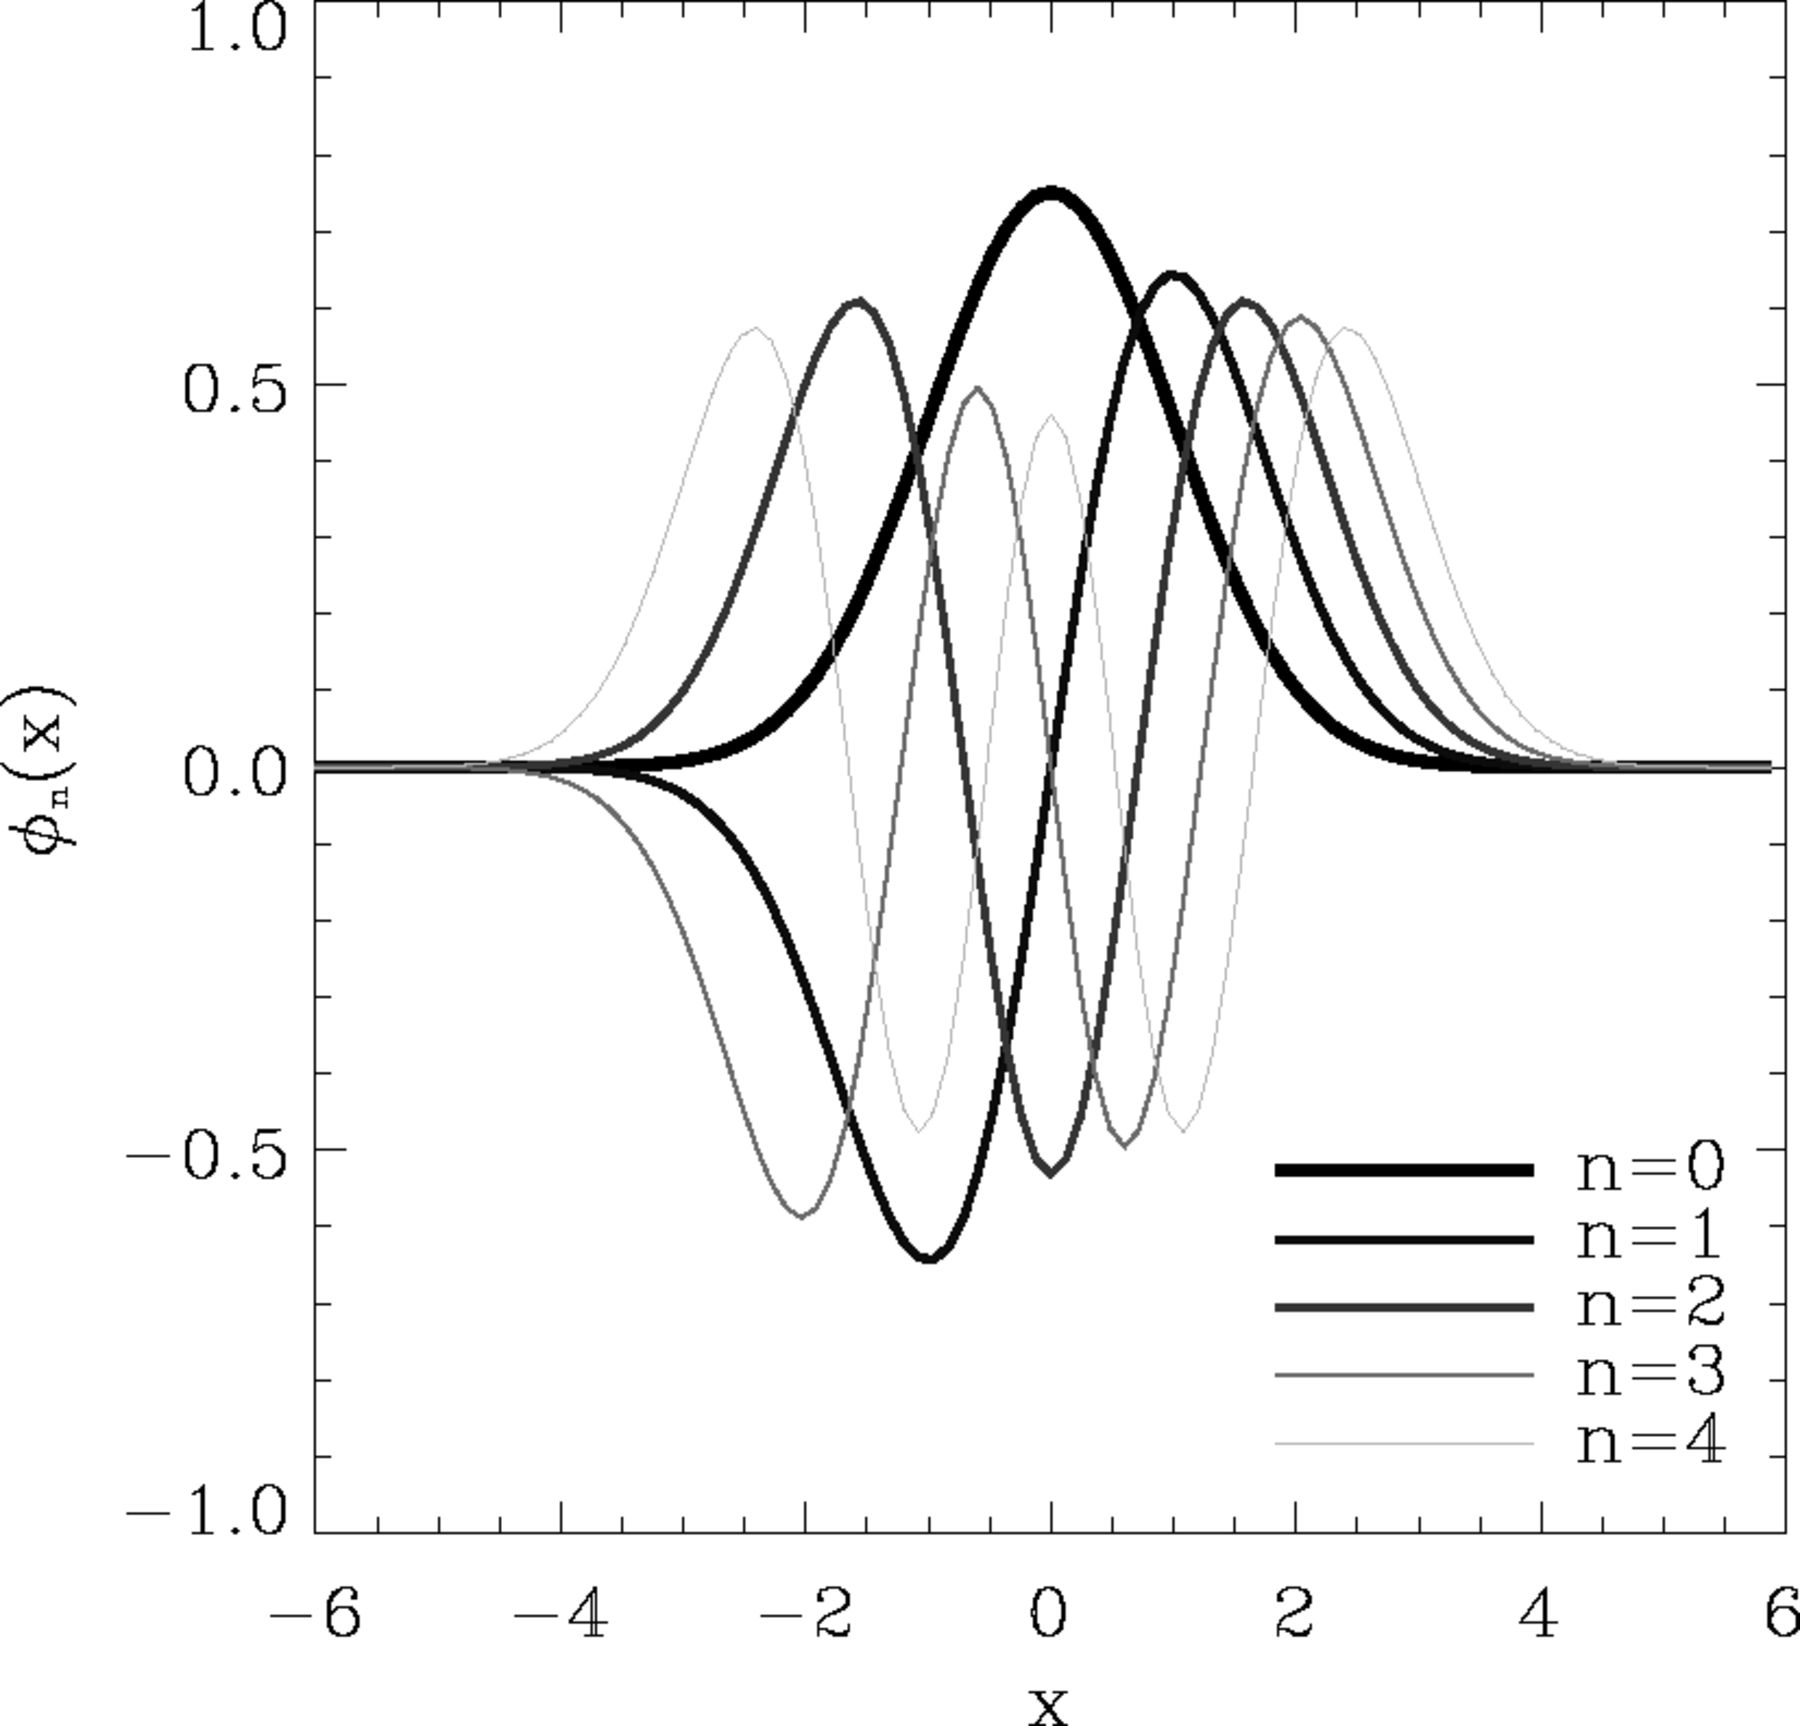
\includegraphics [scale=0.5] {refregier-1}
\caption{Первые несколько одномерных базисных функций $\phi_n(x)$. Взято из \todo{Refregier, 2003, рис. 1}.}
\label{fig:Sh1}
\end{figure}

Для двумерного случая удобно пользоваться представлением:\\
\begin{equation}
\label{eq:shape-basis-functions}
B_{n_1,n_2}(\beta,x,y,x_{ph},y_{ph}) = \beta^{-1}\cdot\phi_{n_1}(\frac{x-x_{ph}}{\beta})\cdot\phi_{n_2}(\frac{y-y_{ph}}{\beta}.
\end{equation}
\\Здесь параметр $\beta$ - характерный размер изображения. В первом приближении его часто приравнивают стандарту двумерной гауссианы при $a=b$. В этом случае хорошей оценкой является $\beta = FWHM/2.35$ ($FWHM$ - ширина профиля звездного изображения на половине максимального отсчета). Индексы $n_1,n_2$ в формуле~\ref{eq:Shbasis-functions}  - порядки полиномов Эрмита по осям $x$ и $y$.

Таким образом изображение может быть представлено в виде:\\
\begin{equation}
\label{eq:image-shapelet}
I(x,y) = I_{bgr}+\sum_{n_1,n_2=0}^{\infty}f_{n_1,n_2}\cdot B_{n_1,n_2}(\beta,x,y,x_{ph},y_{ph}),
\end{equation}
\\где $f_{n_1,n_2}$ коэффициенты шейплет-разложения соответствующих порядков $n_1,n_2$.
Изображения первых нескольких двумерных функций представлены на рис. 20. Опять же, их можно рассматривать как возмущения вокруг двумерной Гауссианы $\phi_{00}$.

\begin{figure}[h]
\centering
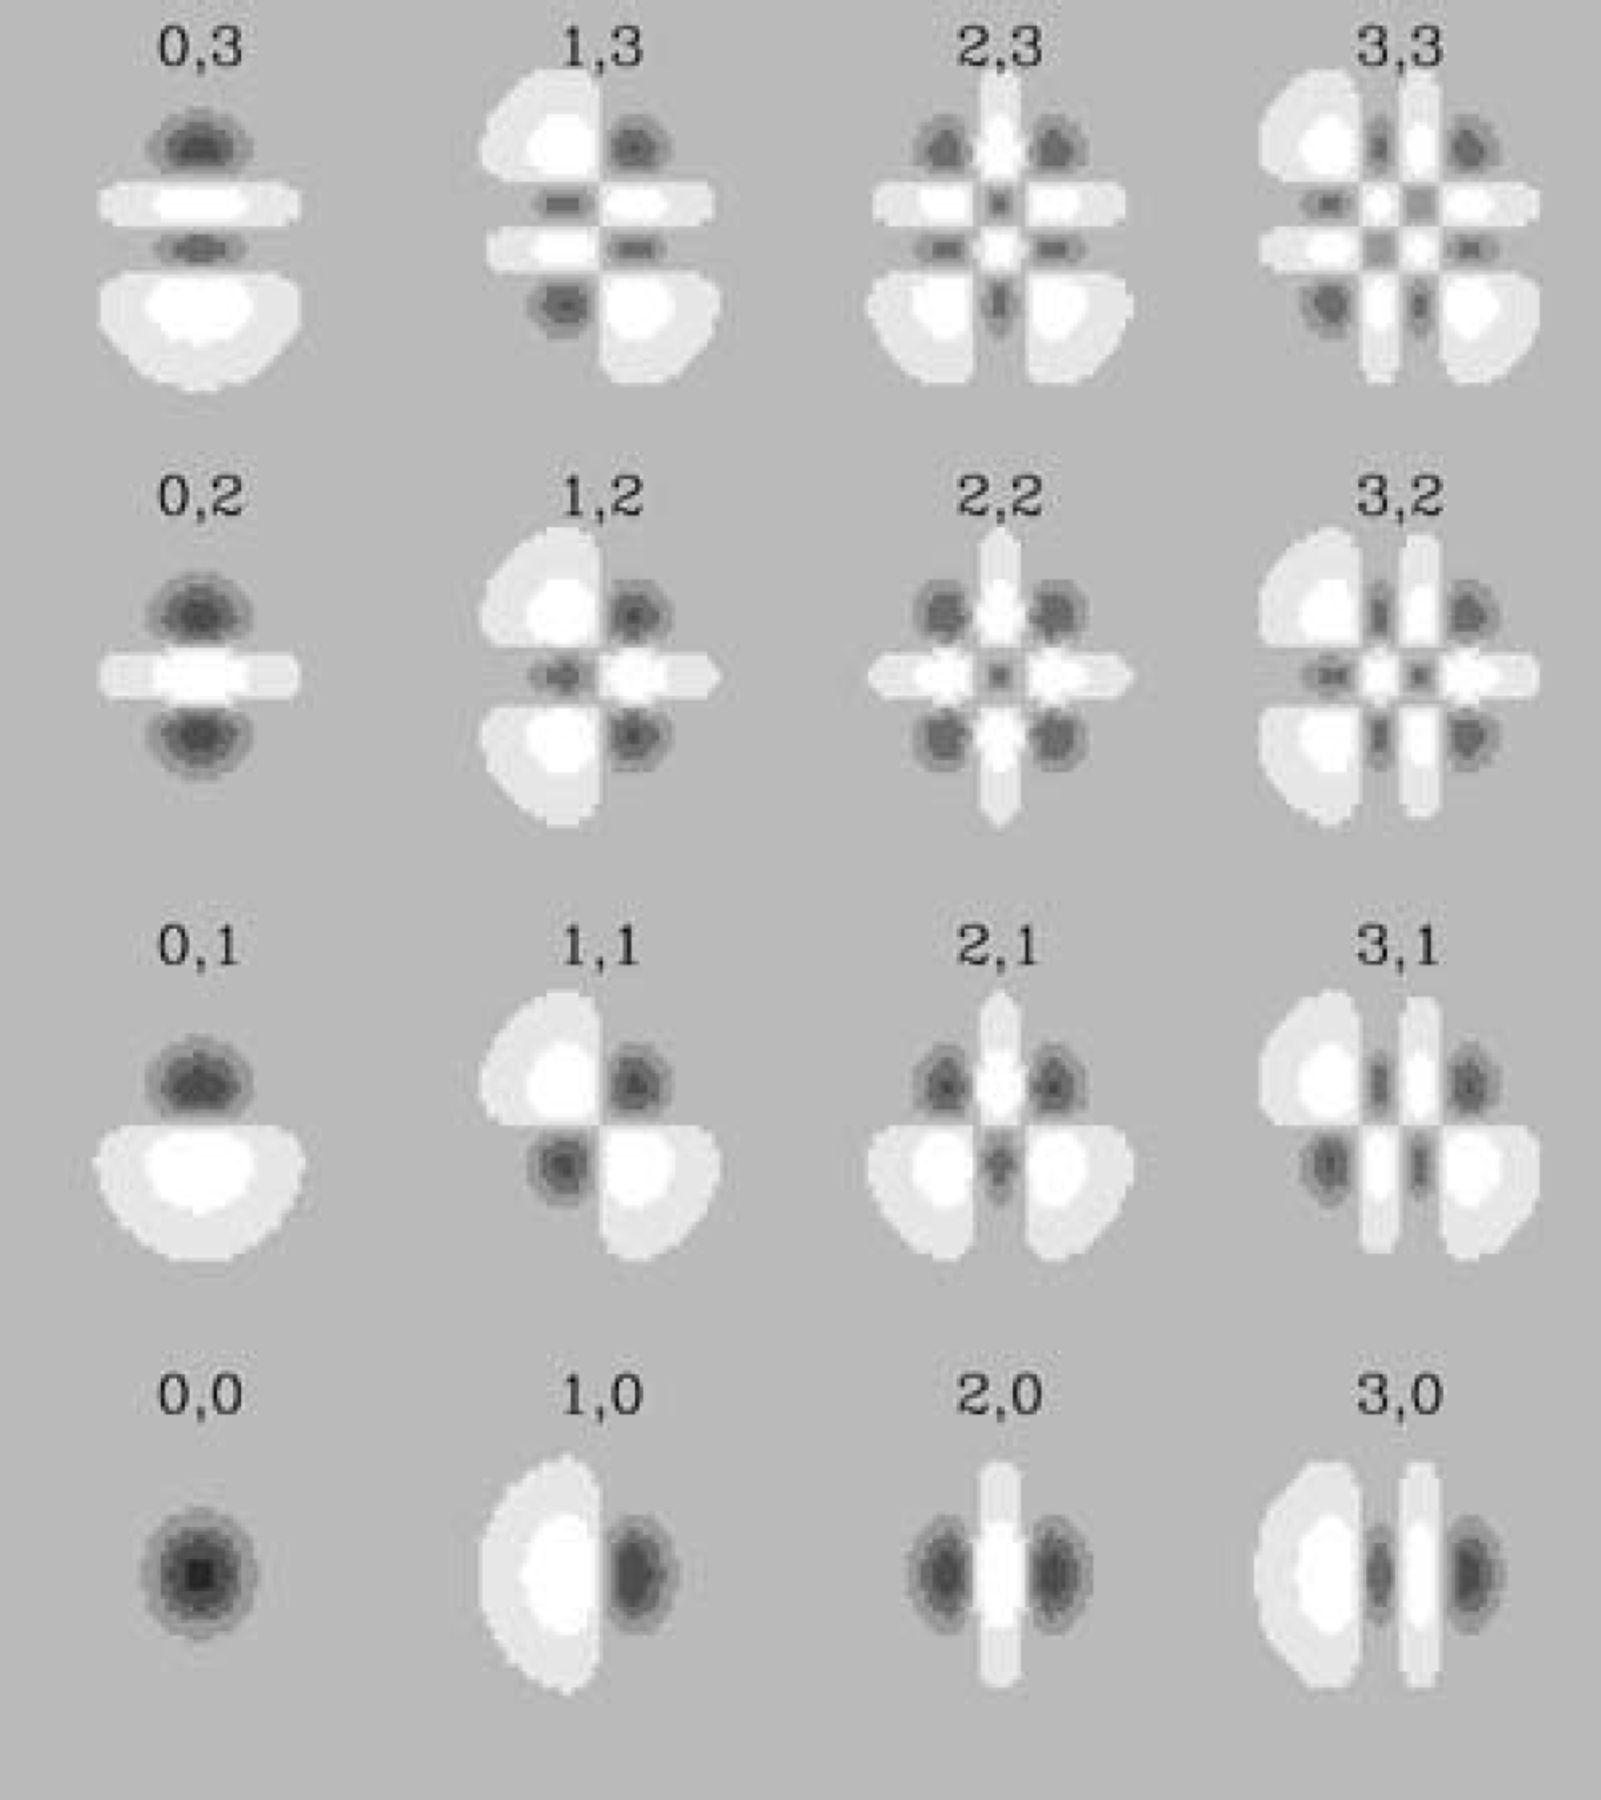
\includegraphics [scale=0.5] {refregier-2}
\caption{Первые несколько двумерных декартовых базисных функций. Темные и светлые области иллюстрируют положительные и отрицательные значения соответственно. Взято из \todo{Refregier, 2003, рис. 2}}
\label{fig:Sh2}
\end{figure}

Несмотря на то, что $B_{n_1,n_2}(\beta,x,y,x_{ph},y_{ph})$ - система ортогональных функций, на практике для оценки $f_{n_1,n_2}$ удобнее пользоваться методом наименьших квадратов. Это связано с тем, что суммирование производится в небольшой области ПЗС-кадра (например 40$\times$40 пикселей). Ряд обрывают при условии $n_1+n_2=n_{max}$, так как при больших $n_1,n_2$ ошибка единицы веса становится меньше стандарта шума изображения. Это значит, что в систему шейплет-коэффициентов проникает информация, характеризующая случайные колебания отсчетов от пикселя к пикселю, а не свойства изображения астрономического объекта. Поэтому приближенное равенство стандарта шума и ошибки единицы веса рассматривается как условие для подбора оптимального значения $n_{max}$.  Примеры аппроксимации изображений одиночной и двойной звезды показаны на рис.~\ref{fig:model-stars} и рис.~\ref{fig:model-bin-stars}. Видно, что при $n_{max}=9$ в результате вычитания модельного изображения из исходного не остается заметной систематической составляющей.

\begin{figure}
%\onelinecaptionsfalse
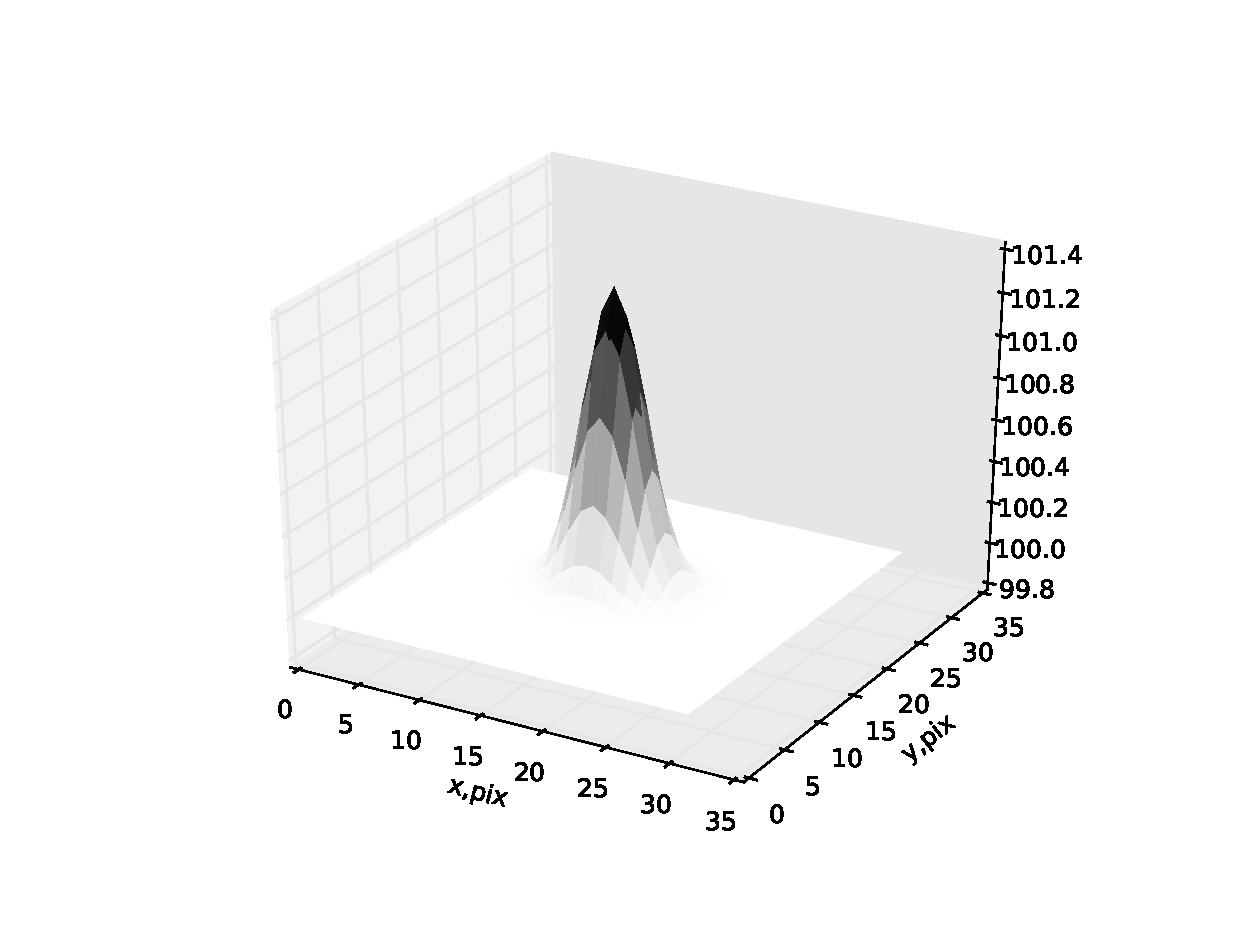
\includegraphics[width=0.4\columnwidth]{stimg_0.eps}
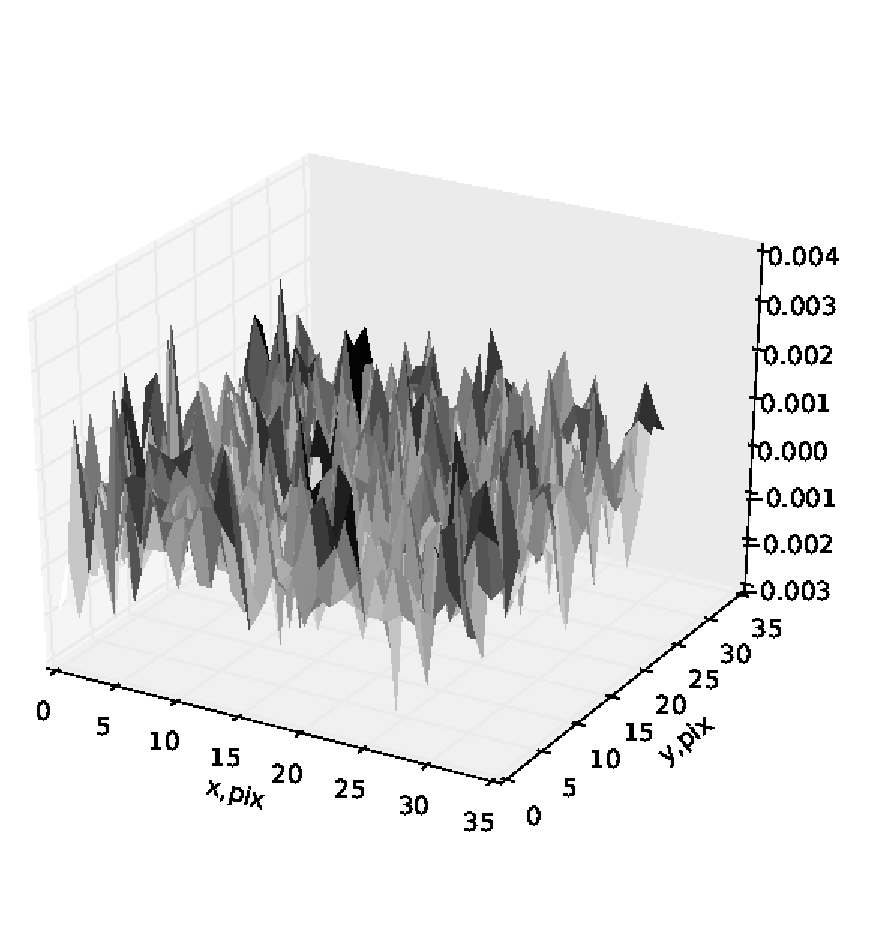
\includegraphics[width=0.4\columnwidth]{res_0.eps}
%\setcaptionmargin{5mm}
%\captionstyle{normal}
\caption{Изображение одиночной звезды (слева) и результат вычитания из реального изображения его модели (справа), построенной посредством shapelet--разложения.}
\label{fig:model-stars}
\end{figure}

\begin{figure}
%\onelinecaptionsfalse
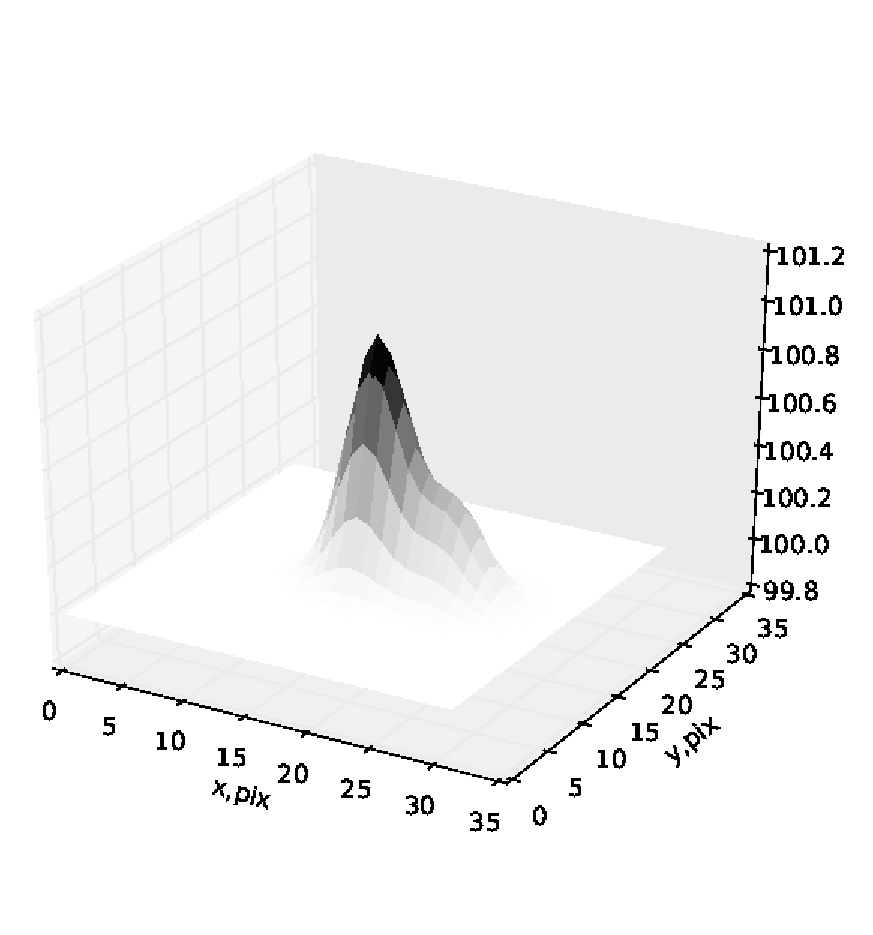
\includegraphics[width=0.4\columnwidth]{stimg_6.eps}
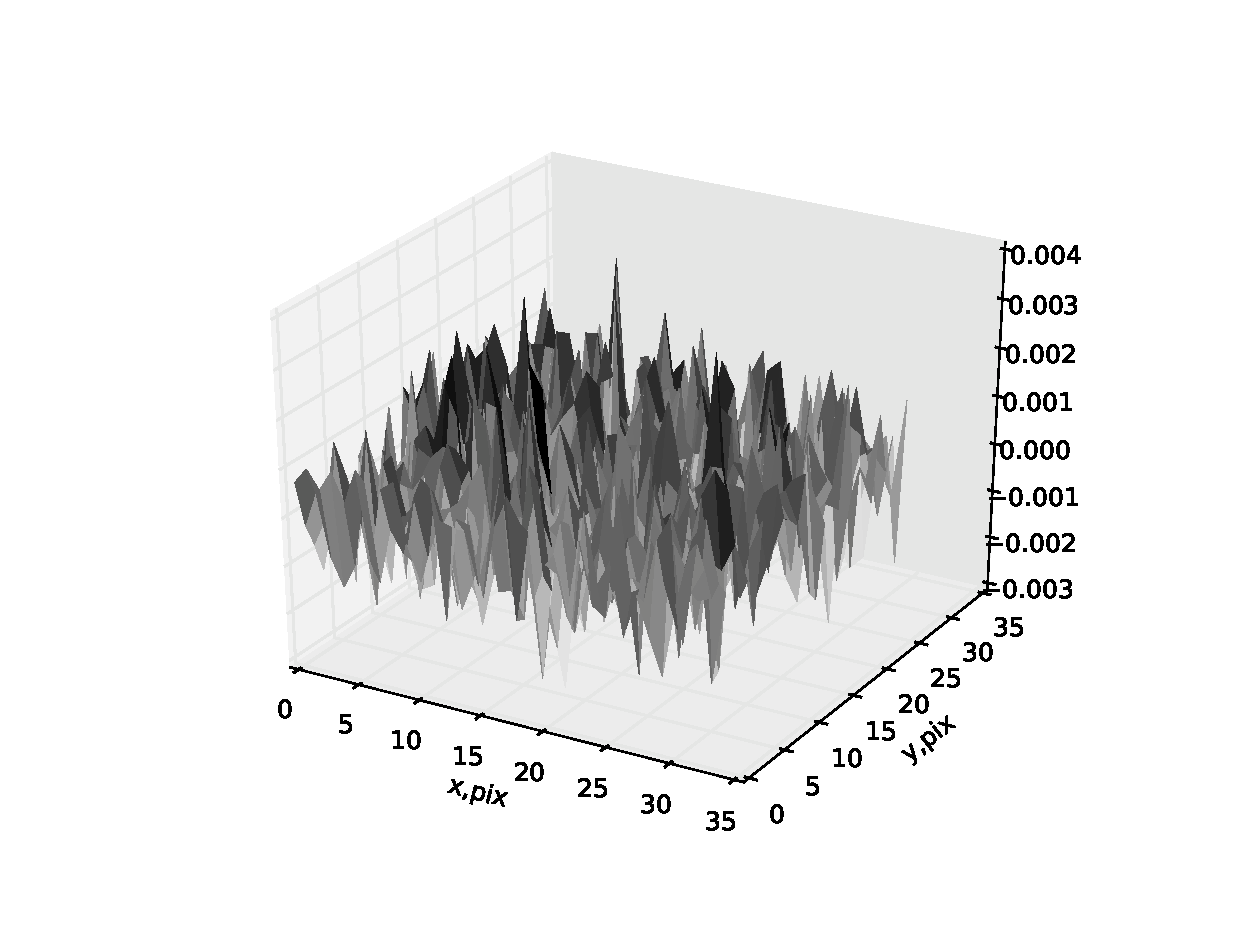
\includegraphics[width=0.4\columnwidth]{res_6.eps}
%\setcaptionmargin{5mm}
%\captionstyle{normal}
\caption{Слева дано изображение двойной звезды ($\Delta m=1^m$, $\rho=6$ pix). Справа "--- результат вычитания из реального изображения его модели2.}
\label{fig:model-bin-stars}
\end{figure}

Привлекательность шейплет--формализма состоит не в только в относительной простоте реализации, но и в том, что многие свойства изображения естественным образом вычисляются на основе коэффициентов разложения $f_{n_1,n_2}$. Так, формула для расчета суммарного потока ($F$) принимает вид:
\begin{equation}
\label{eq:SHFlux}
 F = \sqrt{\pi} \beta \sum^{even}_{n_1,n_2} \sqrt{2^{2-n_1-n_2}C^{\frac{n_1}{2}}_{n_1}C^{\frac{n_2}{2}}_{n_2}}f_{n_1,n_2}
\end{equation}
Здесь \textit{<<even>>} означает, что суммирование выполняется только для четных индексов $n_1,n_2$. $C^{p}_{q}$ - биномиальные коэффициенты для соответствующих индексов.

Положение центра светимости можно выразить формулой:
\begin{equation}
\label{eq:SHPhCent}
x_1^f = \sqrt{\pi} \beta^2 F^{-1} \sum^{odd}_{n_1}\sum^{even}_{n_2} \sqrt{
(n_1+1)2^{2-n_1-n_2}C^{\frac{n_1+1}{2}}_{n_1+1}C^{\frac{n_2}{2}}_{n_2}}f_{n_1,n_2}.
\end{equation}
Здесь \textit{<<odd>>} означает суммирование по нечетным индексам $n_1,n_2$, \textit{<<even>>} "--- по четным. $C^{p}_{q}$ - биномиальные коэффициенты для соответствующих индексов

Также стоит упомянуть, что через shapelet--разложение можно успешно анализировать форму изображения звезд. Это реализуется через квадрупольные моменты изображения,  вычисляемые по формулам:

\begin{align}\label{moments}
 q_{xx} & = F^{-1} \sqrt{\pi} \beta^3 \sum^{even}_{n_1,n_2} (1+2n_1) \sqrt{2^{2-n_1-n_2}C^{\frac{n_1}{2}}_{n_1}C^{\frac{n_2}{2}}_{n_2}}f_{n_1,n_2} \\
 q_{yy} & = F^{-1} \sqrt{\pi} \beta^3 \sum^{even}_{n_1,n_2} (1+2n_2) \sqrt{2^{2-n_1-n_2}C^{\frac{n_1}{2}}_{n_1}C^{\frac{n_2}{2}}_{n_2}}f_{n_1,n_2} \\
 q_{xy} & = F^{-1} \sqrt{\pi} \beta^3 \sum^{odd}_{n_1,n_2} \sqrt{(n_1+1)(n_2+1)2^{2-n_1-n_2}C^{\frac{n_1+1}{2}}_{n_1+1}C^{\frac{n_2+1}{2}}_{n_2+1}}f_{n_1,n_2}
\end{align}

Здесь \textit{<<odd>>} означает суммирование по нечетным индексам.
Более подробно о применении квадрупольных моментов для анализирования формы изображений описаны в Главе 4.

Итак, как мы видим, shapelet--формализм позволяет эффективно решать задачу аппроксимации изображений звезд на сканах астронегативов и ПЗС-кадрах. Для реализации этого подхода в рамках данного исследования разработан соответствующий код на С++ и Python.
